\chapter{Casistica, materiali e metodi}

\section{Casistica}

Sono stati selezionati 29 pazienti (12 maschi e 17 femmine) presso la S.C.D.U. di Auxologia dell'Ospedala Infantile Regina Margherita di Torino. Al fine di ottenere una casistica il più possibile omogenea, si sono adottati i seguenti criteri di inclusione:
\begin{itemize}
\item peso e/o lunghezza alla nascita inferiori al terzo centile secondo gli standarad antropometrici neonatali prodotti dalla task-force della Società Italana di Neonatologia e basati su una popolazione italiana nord-orientale (Figura~\ref{fig:StandardNeonataliNordOccidentali});
\begin{figure}[!h]
  \begin{center}
      \includegraphics{grafici/centili/centili} %\\
  \end{center}
  \caption{Standard antropometrici neonatali relativi a peso ed altezza nell'Italia nord-orientale}
  \label{fig:StandardNeonataliNordOccidentali}
\end{figure}
\item assenza di anomalie cromosomiche (ad esempio sindrome di Turner, Sindrome di Silver Russell), malattie croniche che limitano la crescita (ad esempio insufficienza renale cronica), dismorfismi importanti, displasie scheletriche di rilievo;
\item anamnesi negativa per l'assunzione di farmaci che interferiscono con l'accrescimento (ad esempio corticosteroidi assunti ad alte dosi per un lungo periodo di tempo);
\item assenza di traumi cranici;
\item anamnesi negativa per malnutrizione e disturbi psicosociali;
\item misurazione delle stature di entrambi i genitori con statimetro di Harpenden, ad eccezione dei genitori naturali di due soggetti adottati;
\item diagnosi di deficit di GH secondo le modalità previste dalla nota CUF/AIFA 39 in vigore all'inizio della terapia;
\item trattamento con rGH per almeno 15 mesi consecutivi;
\item raggiungimento della statura finale (quando la velocità di crescita staturale è inferiore ai 2 cm/anno). 
\end{itemize}


\clearpage

% inizio paziente: non segnare il nome ma le prime due lettere di nome e cognome
\subsection*{Paziente 1} % Ma.Va.

Paziente non dismorfico, senza deficit cognitivo, con familiarità per ritardo costituzionale di crescita. 
Cresceva per il limite inferiore del bersaglio parentale.
Ha presentato risposta carente a due test provocativi.

\begin{table}[!h]
\begin{tabular}{lrllrl}
\toprule
\multicolumn{6}{l}{\textbf{Dati alla nascita}}\\
Luogo 		& \multicolumn{2}{l}{Torino} 	& Data 					& \multicolumn{2}{l}{28/12/89} 	\\
Sesso 		& \multicolumn{2}{l}{Femmina} 	& Età gestazionale 		& 40 		& sett.\\
Lunghezza 	& 45 		& cm 				& Centile lunghezza		& $<$ 3° 		\\
Peso 		& 3350 		& g					& Centile peso			& 50° \\
Circonferenza cranica	& 35 		& cm 	& Centile c.c.			& 75° \\
\midrule
\multicolumn{6}{l}{\textbf{Statura dei genitori}}\\
Padre 		& 165,5 & cm 	& Madre 				& 164,2 & cm \\
MPH 		& 158,3 & cm 	& SDS del MPH 			& -0,674\\
\midrule
\multicolumn{6}{l}{\textbf{Inizio trattamento}} \\
Età	& 12,283 & 		& Altezza 				& 135,5 & cm  \\
Centile & $<$ 3° 	 &		& SDS		& -2,054 \\
Velocità di crescita & 4,13 & cm/aa	& Centile di crescita & $<$ 3°\\
\midrule
\multicolumn{6}{l}{\textbf{Trattamento}} \\
Dose media		& 0,77 & UI/kg/sett & Anni prepuberali & 2,5\\
Anni di terapia & 3,6\\
\midrule
\multicolumn{6}{l}{\textbf{Esito della terapia}} \\
Altezza finale			& 157,5 & cm 	& SDS altezza finale		& -0,674\\
SDS dal MPH				& 0 	& 		& SDS guadagnate 			& 1,38\\
\bottomrule
\end{tabular}
\end{table}
\clearpage
% fine paziente. il clear page serve a collocare le tabelle prima del paziente successivo.

% inizio paziente
\subsection*{Paziente 2}% Pa. Gi.

Paziente con ritardo di crescita intrauterino (IUGR) da insufficienza placentare.
Presentava dismorfismi lievi (cubito valgo, clinodattilia lieve, palato ogivale, padiglioni auricolari più grandi della norma) non ascrivibili ad alcuna sindrome genetica. La produzione di GH è risultata carente dopo due test provocativi. Avendo iniziato la pubertà (B2) ad una statura di 120 cm all'età di 10 anni circa, è stata effettuata una terapia combinata con GH biosintetico e LHRH analogo. La terapia con LHRH analogo è stata effettuata per un anno e mezzo circa, fino al raggiungimento di una statura pari a 129,6 cm.

\begin{table}[!h]
\begin{tabular}{lrllrl}
\toprule
\multicolumn{6}{l}{\textbf{Dati alla nascita}}\\
Luogo 		& \multicolumn{2}{l}{Moncalieri} 	& Data 					& \multicolumn{2}{l}{22/04/91} 	\\
Sesso 		& \multicolumn{2}{l}{Femmina} 	& Età gestazionale 		& 41 		& sett.\\
Lunghezza 	& 47 		& cm 				& Centile lunghezza		& 3° -- 10°	\\
Peso 		& 1970 		& g					& Centile peso			& $<$ 3° 		\\
Circonferenza cranica	& 31,6 		& cm 	& Centile c.c.			& $<$ 3° \\
\midrule
\multicolumn{6}{l}{\textbf{Statura dei genitori}}\\
Padre 		& 160,6 & cm 	& Madre 				& 159,4 & cm \\
MPH 		& 153,5 & cm 	& SDS del MPH 			& -1,478\\
\midrule
\multicolumn{6}{l}{\textbf{Inizio trattamento}} \\
Età	& 10,272 & 		& Altezza 				& 121,7 & cm  \\
Centile & $<$ 3° 	 &		& SDS		& -2,5 \\
Velocità di crescita & 2,52 & cm/aa	& Centile di crescita & $<$ 3°\\
\midrule
\multicolumn{6}{l}{\textbf{Trattamento}} \\
Dose media		& 0,79 & UI/kg/sett & Anni prepuberali & 2,6\\
Anni di terapia & 4,6\\
\midrule
\multicolumn{6}{l}{\textbf{Esito della terapia}} \\
Altezza finale			& 147,5 & cm 	& SDS altezza finale & -2,5\\
SDS dal MPH	& -1,022 	& 	& SDS guadagnate 			& 0\\
\bottomrule
\end{tabular}
\end{table}



\clearpage
% fine paziente. il clear page serve a collocare le tabelle prima del paziente successivo.

% inizio paziente
\subsection*{Paziente 3}% Sc. Fl.

Paziente con glaucoma congenito, lieve clinodattilia e familiarità per bassa statura. Ha presentato insufficiente secrezione di GH  dopo due test provocativi.

\marginpar{MPH $<$ 3°, come calcolare SDS guadagnate?}

\begin{table}[!h]
\begin{tabular}{lrllrl}
\toprule
\multicolumn{6}{l}{\textbf{Dati alla nascita}}\\
Luogo 		& \multicolumn{2}{l}{Cirié} 	& Data 					& \multicolumn{2}{l}{07/08/1992} 	\\
Sesso 		& \multicolumn{2}{l}{Femmina} 	& Età gestazionale 		& 39 		& sett.\\
Lunghezza 	& 45,5 		& cm 				& Centile lunghezza		& 3° 		\\
Peso 		& 2570 		& g					& Centile peso			& 3° -- 10° 		\\
Circonferenza cranica	& -- 		& cm 	& Centile c.c.			& -- \\
\midrule
\multicolumn{6}{l}{\textbf{Statura dei genitori}}\\
Padre 		& 158 & cm 		& Madre 				& 139,8 & cm \\
MPH 		& 142,4 & cm 	& SDS del MPH 			& ?? \\
\midrule
\multicolumn{6}{l}{\textbf{Inizio trattamento}} \\
Età	& 8,313 & 		& Altezza 				& 111,6 & cm  \\
Centile & $<$ 3° 	 &		& SDS		& -2,327 \\
Velocità di crescita & 4,05 & cm/aa	& Centile di crescita & $<$ 3°\\
\midrule
\multicolumn{6}{l}{\textbf{Trattamento}} \\
Dose media		& 0,79 & UI/kg/sett & Anni prepuberali & 3,5\\
Anni di terapia & 6\\
\midrule
\multicolumn{6}{l}{\textbf{Esito della terapia}} \\
Altezza finale	& 147,2 & cm 	& SDS altezza finale 	& ??\\
SDS dal MPH	& ?? 	&		& SDS guadagnate 			& ??\\
\bottomrule
\end{tabular}
\end{table}
\clearpage
% fine paziente. il clear page serve a collocare le tabelle prima del paziente successivo.

% inizio paziente
\subsection*{Paziente 4}% Za. Gi.

Paziente non dismorfico, senza deficit cognitivo. La sua produzione di ormone della crescita è risultata deficitaria dopo due test provocativi.

\begin{table}[!h]
\begin{tabular}{lrllrl}
\toprule
\multicolumn{6}{l}{\textbf{Dati alla nascita}}\\
Luogo 		& \multicolumn{2}{l}{Rivoli} 	& Data 					& \multicolumn{2}{l}{24/07/1988} 	\\
Sesso 		& \multicolumn{2}{l}{Maschio} 	& Età gestazionale 		& 41 		& sett.\\
Lunghezza 	& 47 		& cm 				& Centile lunghezza		& $<$ 3° 	\\
Peso 		& 3080 		& g					& Centile peso			& 10° -- 25° 	\\
Circonferenza cranica	& -- 		& cm 	& Centile c.c.			& -- \\
\midrule
\multicolumn{6}{l}{\textbf{Statura dei genitori}}\\
Padre 		& 165,5 & cm 	& Madre 				& 150 & cm \\
MPH 		& 151,2 & cm 	& SDS del MPH 			& -2,5\\
\midrule
\multicolumn{6}{l}{\textbf{Inizio trattamento}} \\
Età	& 14,964 & 		& Altezza 				& 156 & cm  \\
Centile & 3° 	 &		& SDS		& -1,881 \\
Velocità di crescita & 6,88 & cm/aa	& Centile di crescita & 25° -- 50°\\
\midrule
\multicolumn{6}{l}{\textbf{Trattamento}} \\
Dose media		& 0,79 & UI/kg/sett & Anni prepuberali & 0\\
Anni di terapia & 1,5\\
\midrule
\multicolumn{6}{l}{\textbf{Esito della terapia}} \\
Altezza finale			& 166,3 & cm 	& SDS altezza finale		& -0,954\\
SDS dal MPH				& 1,546 &		& SDS guadagnate 			& 0,927\\
\bottomrule
\end{tabular}
\end{table}
\clearpage
% fine paziente. il clear page serve a collocare le tabelle prima del paziente successivo.

% inizio paziente
\subsection*{Paziente 5}% Ze. Lu.

Paziente con brachidattilia (come il padre) e con familiarità per bassa statura. Non presentava dismorfismi. Il picco di ormone della crescita è risultato al di sotto del limite inferiore della norma dopo due test provocativi.

\begin{table}[!h]
\begin{tabular}{lrllrl}
\toprule
\multicolumn{6}{l}{\textbf{Dati alla nascita}}\\
Luogo 		& \multicolumn{2}{l}{Biella} 	& Data 					& \multicolumn{2}{l}{23/11/1991} 	\\
Sesso 		& \multicolumn{2}{l}{Maschio} 	& Età gestazionale 		& 38 		& sett.\\
Lunghezza 	& 45 		& cm 				& Centile lunghezza		& $<$ 3° 		\\
Peso 		& 2650 		& g					& Centile peso			& 10° -- 25° 		\\
Circonferenza cranica	& 33 		& cm 	& Centile c.c.			& 10° -- 25° \\
\midrule
\multicolumn{6}{l}{\textbf{Statura dei genitori}}\\
Padre 		& 161,4 & cm 	& Madre 				& 146,1 & cm \\
MPH 		& 147,2 & cm 	& SDS del MPH 			& ??\\
\midrule
\multicolumn{6}{l}{\textbf{Inizio trattamento}} \\
Età	& 9,877 & 		& Altezza 				& 120,1 & cm  \\
Centile & $<$ 3° 	 &		& SDS		& -2,054 \\
Velocità di crescita & 3,53 & cm/aa	& Centile di crescita & $<$ 3°\\
\midrule
\multicolumn{6}{l}{\textbf{Trattamento}} \\
Dose media		& 0,85 & UI/kg/sett & Anni prepuberali & 3,5\\
Anni di terapia & 5,5\\
\midrule
\multicolumn{6}{l}{\textbf{Esito della terapia}} \\
Altezza finale			& 157 & cm 	& SDS altezza finale		& ??\\
SDS dal MPH				& ?? &		& SDS guadagnate 			& ??\\
\bottomrule
\end{tabular}
\end{table}
\clearpage
% fine paziente. il clear page serve a collocare le tabelle prima del paziente successivo.

% inizio paziente
\subsection*{Paziente 6}% Sa. Ma.

Paziente non dismorfica. Ha presentato arresto di crescita all'età di circa otto anni. La produzione spontanea di GH valutata con dosaggio notturno è risultata carente. Essendo comparso il bottone mammario bilateralmente all'età di 10 anni circa quando la staura era pari a 126,8 cm, è stata proposta la terapia combinata con GH biosintetico e LHRH analogo. Il frenaggio puberale con LHRH analogo ha avuto durata di un anno.   

\begin{table}[h]
\begin{tabular}{lrllrl}
\toprule
\multicolumn{6}{l}{\textbf{Dati alla nascita}}\\
Luogo 		& \multicolumn{2}{l}{Spagna} 	& Data 					& \multicolumn{2}{l}{15/05/1995} 	\\
Sesso 		& \multicolumn{2}{l}{Femmina} 	& Età gestazionale 		& 40 		& sett.\\
Lunghezza 	& 48 		& cm 				& Centile lunghezza		& 10° -- 25° 		\\
Peso 		& 2500 		& g					& Centile peso			& $<$ 3° 		\\
Circonferenza cranica	& -- 		& cm 	& Centile c.c.			& -- \\
\midrule
\multicolumn{6}{l}{\textbf{Statura dei genitori}}\\
Padre 		& 172,8 & cm 	& Madre 				& 143,1 & cm \\
MPH 		& 151,5 & cm 	& SDS del MPH 			& -1,881\\
\midrule
\multicolumn{6}{l}{\textbf{Inizio trattamento}} \\
Età	& 9,7 & 		& Altezza 				& 122 & cm  \\
Centile & $<$ 3° 	 &		& SDS		& -2,327 \\
Velocità di crescita & 4 & cm/aa	& Centile di crescita & $<$ 3°\\
\midrule
\multicolumn{6}{l}{\textbf{Trattamento}} \\
Dose media		& 0,8 & UI/kg/sett & Anni prepuberali & 2,6\\
Anni di terapia & 4,7\\
\midrule
\multicolumn{6}{l}{\textbf{Esito della terapia}} \\
Altezza finale			& 148 & cm 	& SDS altezza finale		& -2,327\\
SDS dal MPH				& -0,446 &		& SDS guadagnate 			& 0\\
\bottomrule
\end{tabular}
\end{table}
\clearpage

\subsection*{Paziente 7}% Co.Be.

Paziente con bassa statura ad esordio prenatale non seguita da crescita di recupero. Presentava lievi dismorfismi non significativi (lieve brevità del collo; arti inferiori leggermente dismorfici). La produzione spontanea di GH valutata con dosaggio notturno si è rivelata deficitaria. Essendo entrata in pubertà a circa 10,5 anni con una di statura poco superiore ai 125 cm, è stata effettuata la terapia combinata con rGH e LHRH analogo. La terapia frenante è stata eseguita per un anno circa. 

\begin{table}[!h]
\begin{tabular}{lrllrl}
\toprule
\multicolumn{6}{l}{\textbf{Dati alla nascita}}\\
Luogo 		& \multicolumn{2}{l}{Torino} 	& Data 					& \multicolumn{2}{l}{15/03/96} 	\\
Sesso 		& \multicolumn{2}{l}{Femmina} 	& Età gestazionale 		& 41 		& sett.\\
Lunghezza 	& 46 		& cm 				& Centile lunghezza		& $<$ 3° 		\\
Peso 		& 2610 		& g					& Centile peso			& $<$ 3° 		\\
Circonferenza cranica	& 32 		& cm 	& Centile c.c.			& 3° \\
\midrule
\multicolumn{6}{l}{\textbf{Statura dei genitori}}\\
Padre 		& 165,7 & cm 	& Madre 				& 161,2 & cm \\
MPH 		& 156,9 & cm 	& SDS del MPH 			& -0,954\\
\midrule
\multicolumn{6}{l}{\textbf{Inizio trattamento}} \\
Età	& 10,7 & 		& Altezza 				& 125,9 & cm  \\
Centile & $<$ 3° 	 &		& SDS		& -2,327 \\
Velocità di crescita & 5,4 & cm/aa	& Centile di crescita & 25°\\
\midrule
\multicolumn{6}{l}{\textbf{Trattamento}} \\
Dose media		& 0,74 & UI/kg/sett & Anni prepuberali & 2\\
Anni di terapia & 3,5\\
\midrule
\multicolumn{6}{l}{\textbf{Esito della terapia}} \\
Altezza finale			& 155,6 & cm 	& SDS altezza finale		& -0,954\\
SDS dal MPH				& 0 &		& SDS guadagnate 			& 1,373\\
\bottomrule
\end{tabular}
\end{table}
\clearpage

\subsection*{Paziente 8}% Ri.El.

\marginpar{come ha avuto accesso alla terapia con rGH?}

Paziente con labioschisi operata all'età di tre mesi. Presentava lievi dimorfismi (padiglioni auricolari piccoli, prognatismo). Dalla nascita aveva rigidità articolare. Essendo stata diagnosticata una lieve stenosi aortica, è stato valutato il cariotipo per sospetta sindrome di Turner. Il risultato non ha confermato l'ipotesi diagnostica. La paziente persentava lieve ritardo psicomotorio. 
Avendo iniziato la pubertà (stadio B2) all'età di 9,4 anni con una statura pari a 122 cm, è stata proposta la terapia frenante associata all'assunzione di rGH. La terapia frenante è stata effettuata per due anni.

\marginpar{esito molto sotto il 3°: come calcolare SDS?}

\begin{table}[!h]
\begin{tabular}{lrllrl}
\toprule
\multicolumn{6}{l}{\textbf{Dati alla nascita}}\\
Luogo 		& \multicolumn{2}{l}{Cuneo} 	& Data 					& \multicolumn{2}{l}{02/01/1986} 	\\
Sesso 		& \multicolumn{2}{l}{Femmina} 	& Età gestazionale 		& 37 		& sett.\\
Lunghezza 	& 43,5 		& cm 				& Centile lunghezza		& $<$ 3° 		\\
Peso 		& 2150 		& g					& Centile peso			& 3° -- 10°		\\
Circonferenza cranica	& -- 		& cm 	& Centile c.c.			& -- \\
\midrule
\multicolumn{6}{l}{\textbf{Statura dei genitori}}\\
Padre 		& 177 & cm 	& Madre 				& 162,6 & cm \\
MPH 		& 163,3 & cm 	& SDS del MPH 			& 0\\
\midrule
\multicolumn{6}{l}{\textbf{Inizio trattamento}} \\
Età	& 10,9 & 		& Altezza 				& 129,8 & cm  \\
Centile & $~$ 3°	 &		& SDS		& -1,881 \\
Velocità di crescita & 3,33 & cm/a	& Centile di crescita & $<$ 3°\\
\midrule
\multicolumn{6}{l}{\textbf{Trattamento}} \\
Dose media		& 0,8 & UI/kg/sett & Anni prepuberali & 0,6\\
Anni di terapia & 2,6\\
\midrule
\multicolumn{6}{l}{\textbf{Esito della terapia}} \\
Altezza finale			& 144,7 & cm 	& SDS altezza finale		& ??\\
SDS dal MPH				& ?? &		& SDS guadagnate 			& ??\\
\bottomrule
\end{tabular}
\end{table}
\clearpage


\subsection*{Paziente 9}% Mu. El.

\marginpar{come ha avuto accesso alla terapia con rGH ?}

Soggetto affetto da strabismo, con familiarità per bassa statura. La paziente è sempre cresciuta lentamente.

\marginpar{in realtà avrebbe guadagnato qualcosina, ma come valutarne l'SDS}

\begin{table}[!h]
\begin{tabular}{lrllrl}
\toprule
\multicolumn{6}{l}{\textbf{Dati alla nascita}}\\
Luogo 		& \multicolumn{2}{l}{Alba} 	& Data 					& \multicolumn{2}{l}{01/10/1985} 	\\
Sesso 		& \multicolumn{2}{l}{Femmina} 	& Età gestazionale 		& 41 		& sett.\\
Lunghezza 	& 46 		& cm 				& Centile lunghezza		& $<$ 3° 		\\
Peso 		& 2260 		& g					& Centile peso			& $<$ 3° 		\\
Circonferenza cranica	& -- 		& cm 	& Centile c.c.			& -- \\
\midrule
\multicolumn{6}{l}{\textbf{Statura dei genitori}}\\
Padre 		& 163,2 & cm 	& Madre 				& 142,6 & cm \\
MPH 		& 146,4 & cm 	& SDS del MPH 			& -2,5\\
\midrule
\multicolumn{6}{l}{\textbf{Inizio trattamento}} \\
Età	& 11,561 & 		& Altezza 				& 122,6 & cm  \\
Centile & $<$ 3° 	 &		& SDS		& -2,5 \\
Velocità di crescita & 3,7 & cm/a	& Centile di crescita & $<$ 3°\\
\midrule
\multicolumn{6}{l}{\textbf{Trattamento}} \\
Dose media		& 0,98 & UI/kg/sett & Anni prepuberali & 3,5\\
Anni di terapia & 4\\
\midrule
\multicolumn{6}{l}{\textbf{Esito della terapia}} \\
Altezza finale			& 146,8 & cm 	& SDS altezza finale		& -2,5\\
SDS dal MPH				& 0 &		& SDS guadagnate 			& 0\\
\bottomrule
\end{tabular}
\end{table}
\clearpage


\subsection*{Paziente 10}%  Ba. Ma.

Paziente adottata. La madre naturale era tossicodipendente, affetta da HBV. Probabilmente entrambi i genitori naturali erano di bassa statura. La bambina è nata con Sindrome da Distress Respiratorio e sindrome da astinenza. Non ha mai presentato ritardo psicomotorio. La produzione di ormone somatotropo è risultata deficitaria dopo due test di stimolo.

\begin{table}[!h]
\begin{tabular}{lrllrl}
\toprule
\multicolumn{6}{l}{\textbf{Dati alla nascita}}\\
Luogo 		& \multicolumn{2}{l}{Torino} 	& Data 					& \multicolumn{2}{l}{02/07/1988} 	\\
Sesso 		& \multicolumn{2}{l}{Femmina} 	& Età gestazionale 		& 27 		& sett.\\
Lunghezza 	& 31,5 		& cm 				& Centile lunghezza		& 3° 		\\
Peso 		& 700 		& g					& Centile peso			& 10° -- 25° \\
Circonferenza cranica	& -- 		& cm 	& Centile c.c.			& -- \\
\midrule
\multicolumn{6}{l}{\textbf{Statura dei genitori}}\\
Padre 		& -- &  	& Madre 				& -- &  \\
MPH 		& -- & cm 	& SDS del MPH 			& --\\
\midrule
\multicolumn{6}{l}{\textbf{Inizio trattamento}} \\
Età	& 6,372 & 		& Altezza 				& 97,6 & cm  \\
Centile & $<$ 3° 	 &		& SDS		& -2,5 \\
Velocità di crescita & 5,4 & cm/a	& Centile di crescita & 25°\\
\midrule
\multicolumn{6}{l}{\textbf{Trattamento}} \\
Dose media		& 0,91 & UI/kg/sett & Anni prepuberali & 0,6\\
Anni di terapia & 7,6\\
\midrule
\multicolumn{6}{l}{\textbf{Esito della terapia}} \\
Altezza finale			& 160,8 & cm 	& SDS altezza finale		& -0,050\\
SDS dal MPH				& -- &		& SDS guadagnate 			& 2,45\\
\bottomrule
\end{tabular}
\end{table}
\clearpage


\subsection*{Paziente 11}% Pe. Sa.

\marginpar{come ha avuto accesso alla terapia con rGH ?}

Soggetto IUGR. Il ritardo di crescita è stato rilevato ecograficamente al settimo mese di gravidanza. La causa è sconosciuta; probabilmente la madre aveva assunto farmaci. La bambina è stata operata a quattro anni di età per chiudere il difetto inter-atriale presente alla nascita. A nove giorni di vita ha manifestato convulsioni di natura da detrminarsi: la TC esguita era negativa. LA bambina presentava lievi dimorfismi: impianto basso dei padiglioni auricolari, sindattilia, capigliatura scarsa, strabismo, epicanto, pterigio, brevità del primo metacarpo sinistro. Pertanto è stata effettuata la mappa cromosomica, ma non sono emerse alterazioni.   



\begin{table}[!h]
\begin{tabular}{lrllrl}
\toprule
\multicolumn{6}{l}{\textbf{Dati alla nascita}}\\
Luogo 		& \multicolumn{2}{l}{??} 	& Data 					& \multicolumn{2}{l}{??} 	\\
Sesso 		& \multicolumn{2}{l}{??} 	& Età gestazionale 		& ?? 		& sett.\\
Lunghezza 	& ?? 		& cm 				& Centile lunghezza		& ?? 		\\
Peso 		& ?? 		& g					& Centile peso			& ?? 		\\
Circonferenza cranica	& ?? 		& cm 	& Centile c.c.			& ?? \\
\midrule
\multicolumn{6}{l}{\textbf{Statura dei genitori}}\\
Padre 		& ?? & cm 	& Madre 				& ?? & cm \\
MPH 		& ?? & cm 	& SDS del MPH 			& ??\\
\midrule
\multicolumn{6}{l}{\textbf{Inizio trattamento}} \\
Età	& ?? & 		& Altezza 				& ?? & cm  \\
Centile & ?? 	 &		& SDS		& ?? \\
Velocità di crescita & ?? & cm/a	& Centile di crescita & ??\\
\midrule
\multicolumn{6}{l}{\textbf{Trattamento}} \\
Dose media		& ?? & UI/kg/sett & Anni prepuberali & ??\\
Anni di terapia & ??\\
\midrule
\multicolumn{6}{l}{\textbf{Esito della terapia}} \\
Altezza finale			& ?? & cm 	& SDS altezza finale		& ??\\
SDS dal MPH				& ?? &		& SDS guadagnate 			& ??\\
\bottomrule
\end{tabular}
\end{table}
\clearpage


\subsection*{Paziente 12}

TODO

\begin{table}[!h]
\begin{tabular}{lrllrl}
\toprule
\multicolumn{6}{l}{\textbf{Dati alla nascita}}\\
Luogo 		& \multicolumn{2}{l}{??} 	& Data 					& \multicolumn{2}{l}{??} 	\\
Sesso 		& \multicolumn{2}{l}{??} 	& Età gestazionale 		& ?? 		& sett.\\
Lunghezza 	& ?? 		& cm 				& Centile lunghezza		& ?? 		\\
Peso 		& ?? 		& g					& Centile peso			& ?? 		\\
Circonferenza cranica	& ?? 		& cm 	& Centile c.c.			& ?? \\
\midrule
\multicolumn{6}{l}{\textbf{Statura dei genitori}}\\
Padre 		& ?? & cm 	& Madre 				& ?? & cm \\
MPH 		& ?? & cm 	& SDS del MPH 			& ??\\
\midrule
\multicolumn{6}{l}{\textbf{Inizio trattamento}} \\
Età	& ?? & 		& Altezza 				& ?? & cm  \\
Centile & ?? 	 &		& SDS		& ?? \\
Velocità di crescita & ?? & cm/a	& Centile di crescita & ??\\
\midrule
\multicolumn{6}{l}{\textbf{Trattamento}} \\
Dose media		& ?? & UI/kg/sett & Anni prepuberali & ??\\
Anni di terapia & ??\\
\midrule
\multicolumn{6}{l}{\textbf{Esito della terapia}} \\
Altezza finale			& ?? & cm 	& SDS altezza finale		& ??\\
SDS dal MPH				& ?? &		& SDS guadagnate 			& ??\\
\bottomrule
\end{tabular}
\end{table}
\clearpage


\subsection*{Paziente 13}

TODO

\begin{table}[!h]
\begin{tabular}{lrllrl}
\toprule
\multicolumn{6}{l}{\textbf{Dati alla nascita}}\\
Luogo 		& \multicolumn{2}{l}{??} 	& Data 					& \multicolumn{2}{l}{??} 	\\
Sesso 		& \multicolumn{2}{l}{??} 	& Età gestazionale 		& ?? 		& sett.\\
Lunghezza 	& ?? 		& cm 				& Centile lunghezza		& ?? 		\\
Peso 		& ?? 		& g					& Centile peso			& ?? 		\\
Circonferenza cranica	& ?? 		& cm 	& Centile c.c.			& ?? \\
\midrule
\multicolumn{6}{l}{\textbf{Statura dei genitori}}\\
Padre 		& ?? & cm 	& Madre 				& ?? & cm \\
MPH 		& ?? & cm 	& SDS del MPH 			& ??\\
\midrule
\multicolumn{6}{l}{\textbf{Inizio trattamento}} \\
Età	& ?? & 		& Altezza 				& ?? & cm  \\
Centile & ?? 	 &		& SDS		& ?? \\
Velocità di crescita & ?? & cm/a	& Centile di crescita & ??\\
\midrule
\multicolumn{6}{l}{\textbf{Trattamento}} \\
Dose media		& ?? & UI/kg/sett & Anni prepuberali & ??\\
Anni di terapia & ??\\
\midrule
\multicolumn{6}{l}{\textbf{Esito della terapia}} \\
Altezza finale			& ?? & cm 	& SDS altezza finale		& ??\\
SDS dal MPH				& ?? &		& SDS guadagnate 			& ??\\
\bottomrule
\end{tabular}
\end{table}
\clearpage


\subsection*{Paziente 14}

TODO

\begin{table}[!h]
\begin{tabular}{lrllrl}
\toprule
\multicolumn{6}{l}{\textbf{Dati alla nascita}}\\
Luogo 		& \multicolumn{2}{l}{??} 	& Data 					& \multicolumn{2}{l}{??} 	\\
Sesso 		& \multicolumn{2}{l}{??} 	& Età gestazionale 		& ?? 		& sett.\\
Lunghezza 	& ?? 		& cm 				& Centile lunghezza		& ?? 		\\
Peso 		& ?? 		& g					& Centile peso			& ?? 		\\
Circonferenza cranica	& ?? 		& cm 	& Centile c.c.			& ?? \\
\midrule
\multicolumn{6}{l}{\textbf{Statura dei genitori}}\\
Padre 		& ?? & cm 	& Madre 				& ?? & cm \\
MPH 		& ?? & cm 	& SDS del MPH 			& ??\\
\midrule
\multicolumn{6}{l}{\textbf{Inizio trattamento}} \\
Età	& ?? & 		& Altezza 				& ?? & cm  \\
Centile & ?? 	 &		& SDS		& ?? \\
Velocità di crescita & ?? & cm/a	& Centile di crescita & ??\\
\midrule
\multicolumn{6}{l}{\textbf{Trattamento}} \\
Dose media		& ?? & UI/kg/sett & Anni prepuberali & ??\\
Anni di terapia & ??\\
\midrule
\multicolumn{6}{l}{\textbf{Esito della terapia}} \\
Altezza finale			& ?? & cm 	& SDS altezza finale		& ??\\
SDS dal MPH				& ?? &		& SDS guadagnate 			& ??\\
\bottomrule
\end{tabular}
\end{table}
\clearpage


\subsection*{Paziente 15}

TODO

\begin{table}[!h]
\begin{tabular}{lrllrl}
\toprule
\multicolumn{6}{l}{\textbf{Dati alla nascita}}\\
Luogo 		& \multicolumn{2}{l}{??} 	& Data 					& \multicolumn{2}{l}{??} 	\\
Sesso 		& \multicolumn{2}{l}{??} 	& Età gestazionale 		& ?? 		& sett.\\
Lunghezza 	& ?? 		& cm 				& Centile lunghezza		& ?? 		\\
Peso 		& ?? 		& g					& Centile peso			& ?? 		\\
Circonferenza cranica	& ?? 		& cm 	& Centile c.c.			& ?? \\
\midrule
\multicolumn{6}{l}{\textbf{Statura dei genitori}}\\
Padre 		& ?? & cm 	& Madre 				& ?? & cm \\
MPH 		& ?? & cm 	& SDS del MPH 			& ??\\
\midrule
\multicolumn{6}{l}{\textbf{Inizio trattamento}} \\
Età	& ?? & 		& Altezza 				& ?? & cm  \\
Centile & ?? 	 &		& SDS		& ?? \\
Velocità di crescita & ?? & cm/a	& Centile di crescita & ??\\
\midrule
\multicolumn{6}{l}{\textbf{Trattamento}} \\
Dose media		& ?? & UI/kg/sett & Anni prepuberali & ??\\
Anni di terapia & ??\\
\midrule
\multicolumn{6}{l}{\textbf{Esito della terapia}} \\
Altezza finale			& ?? & cm 	& SDS altezza finale		& ??\\
SDS dal MPH				& ?? &		& SDS guadagnate 			& ??\\
\bottomrule
\end{tabular}
\end{table}
\clearpage


\subsection*{Paziente 16}

TODO

\begin{table}[!h]
\begin{tabular}{lrllrl}
\toprule
\multicolumn{6}{l}{\textbf{Dati alla nascita}}\\
Luogo 		& \multicolumn{2}{l}{??} 	& Data 					& \multicolumn{2}{l}{??} 	\\
Sesso 		& \multicolumn{2}{l}{??} 	& Età gestazionale 		& ?? 		& sett.\\
Lunghezza 	& ?? 		& cm 				& Centile lunghezza		& ?? 		\\
Peso 		& ?? 		& g					& Centile peso			& ?? 		\\
Circonferenza cranica	& ?? 		& cm 	& Centile c.c.			& ?? \\
\midrule
\multicolumn{6}{l}{\textbf{Statura dei genitori}}\\
Padre 		& ?? & cm 	& Madre 				& ?? & cm \\
MPH 		& ?? & cm 	& SDS del MPH 			& ??\\
\midrule
\multicolumn{6}{l}{\textbf{Inizio trattamento}} \\
Età	& ?? & 		& Altezza 				& ?? & cm  \\
Centile & ?? 	 &		& SDS		& ?? \\
Velocità di crescita & ?? & cm/a	& Centile di crescita & ??\\
\midrule
\multicolumn{6}{l}{\textbf{Trattamento}} \\
Dose media		& ?? & UI/kg/sett & Anni prepuberali & ??\\
Anni di terapia & ??\\
\midrule
\multicolumn{6}{l}{\textbf{Esito della terapia}} \\
Altezza finale			& ?? & cm 	& SDS altezza finale		& ??\\
SDS dal MPH				& ?? &		& SDS guadagnate 			& ??\\
\bottomrule
\end{tabular}
\end{table}
\clearpage


\subsection*{Paziente 17}

TODO

\begin{table}[!h]
\begin{tabular}{lrllrl}
\toprule
\multicolumn{6}{l}{\textbf{Dati alla nascita}}\\
Luogo 		& \multicolumn{2}{l}{??} 	& Data 					& \multicolumn{2}{l}{??} 	\\
Sesso 		& \multicolumn{2}{l}{??} 	& Età gestazionale 		& ?? 		& sett.\\
Lunghezza 	& ?? 		& cm 				& Centile lunghezza		& ?? 		\\
Peso 		& ?? 		& g					& Centile peso			& ?? 		\\
Circonferenza cranica	& ?? 		& cm 	& Centile c.c.			& ?? \\
\midrule
\multicolumn{6}{l}{\textbf{Statura dei genitori}}\\
Padre 		& ?? & cm 	& Madre 				& ?? & cm \\
MPH 		& ?? & cm 	& SDS del MPH 			& ??\\
\midrule
\multicolumn{6}{l}{\textbf{Inizio trattamento}} \\
Età	& ?? & 		& Altezza 				& ?? & cm  \\
Centile & ?? 	 &		& SDS		& ?? \\
Velocità di crescita & ?? & cm/a	& Centile di crescita & ??\\
\midrule
\multicolumn{6}{l}{\textbf{Trattamento}} \\
Dose media		& ?? & UI/kg/sett & Anni prepuberali & ??\\
Anni di terapia & ??\\
\midrule
\multicolumn{6}{l}{\textbf{Esito della terapia}} \\
Altezza finale			& ?? & cm 	& SDS altezza finale		& ??\\
SDS dal MPH				& ?? &		& SDS guadagnate 			& ??\\
\bottomrule
\end{tabular}
\end{table}
\clearpage


\subsection*{Paziente 18}

TODO

\begin{table}[!h]
\begin{tabular}{lrllrl}
\toprule
\multicolumn{6}{l}{\textbf{Dati alla nascita}}\\
Luogo 		& \multicolumn{2}{l}{??} 	& Data 					& \multicolumn{2}{l}{??} 	\\
Sesso 		& \multicolumn{2}{l}{??} 	& Età gestazionale 		& ?? 		& sett.\\
Lunghezza 	& ?? 		& cm 				& Centile lunghezza		& ?? 		\\
Peso 		& ?? 		& g					& Centile peso			& ?? 		\\
Circonferenza cranica	& ?? 		& cm 	& Centile c.c.			& ?? \\
\midrule
\multicolumn{6}{l}{\textbf{Statura dei genitori}}\\
Padre 		& ?? & cm 	& Madre 				& ?? & cm \\
MPH 		& ?? & cm 	& SDS del MPH 			& ??\\
\midrule
\multicolumn{6}{l}{\textbf{Inizio trattamento}} \\
Età	& ?? & 		& Altezza 				& ?? & cm  \\
Centile & ?? 	 &		& SDS		& ?? \\
Velocità di crescita & ?? & cm/a	& Centile di crescita & ??\\
\midrule
\multicolumn{6}{l}{\textbf{Trattamento}} \\
Dose media		& ?? & UI/kg/sett & Anni prepuberali & ??\\
Anni di terapia & ??\\
\midrule
\multicolumn{6}{l}{\textbf{Esito della terapia}} \\
Altezza finale			& ?? & cm 	& SDS altezza finale		& ??\\
SDS dal MPH				& ?? &		& SDS guadagnate 			& ??\\
\bottomrule
\end{tabular}
\end{table}
\clearpage


\subsection*{Paziente 19}

TODO

\begin{table}[!h]
\begin{tabular}{lrllrl}
\toprule
\multicolumn{6}{l}{\textbf{Dati alla nascita}}\\
Luogo 		& \multicolumn{2}{l}{??} 	& Data 					& \multicolumn{2}{l}{??} 	\\
Sesso 		& \multicolumn{2}{l}{??} 	& Età gestazionale 		& ?? 		& sett.\\
Lunghezza 	& ?? 		& cm 				& Centile lunghezza		& ?? 		\\
Peso 		& ?? 		& g					& Centile peso			& ?? 		\\
Circonferenza cranica	& ?? 		& cm 	& Centile c.c.			& ?? \\
\midrule
\multicolumn{6}{l}{\textbf{Statura dei genitori}}\\
Padre 		& ?? & cm 	& Madre 				& ?? & cm \\
MPH 		& ?? & cm 	& SDS del MPH 			& ??\\
\midrule
\multicolumn{6}{l}{\textbf{Inizio trattamento}} \\
Età	& ?? & 		& Altezza 				& ?? & cm  \\
Centile & ?? 	 &		& SDS		& ?? \\
Velocità di crescita & ?? & cm/a	& Centile di crescita & ??\\
\midrule
\multicolumn{6}{l}{\textbf{Trattamento}} \\
Dose media		& ?? & UI/kg/sett & Anni prepuberali & ??\\
Anni di terapia & ??\\
\midrule
\multicolumn{6}{l}{\textbf{Esito della terapia}} \\
Altezza finale			& ?? & cm 	& SDS altezza finale		& ??\\
SDS dal MPH				& ?? &		& SDS guadagnate 			& ??\\
\bottomrule
\end{tabular}
\end{table}
\clearpage


\subsection*{Paziente 20}

TODO

\begin{table}[!h]
\begin{tabular}{lrllrl}
\toprule
\multicolumn{6}{l}{\textbf{Dati alla nascita}}\\
Luogo 		& \multicolumn{2}{l}{??} 	& Data 					& \multicolumn{2}{l}{??} 	\\
Sesso 		& \multicolumn{2}{l}{??} 	& Età gestazionale 		& ?? 		& sett.\\
Lunghezza 	& ?? 		& cm 				& Centile lunghezza		& ?? 		\\
Peso 		& ?? 		& g					& Centile peso			& ?? 		\\
Circonferenza cranica	& ?? 		& cm 	& Centile c.c.			& ?? \\
\midrule
\multicolumn{6}{l}{\textbf{Statura dei genitori}}\\
Padre 		& ?? & cm 	& Madre 				& ?? & cm \\
MPH 		& ?? & cm 	& SDS del MPH 			& ??\\
\midrule
\multicolumn{6}{l}{\textbf{Inizio trattamento}} \\
Età	& ?? & 		& Altezza 				& ?? & cm  \\
Centile & ?? 	 &		& SDS		& ?? \\
Velocità di crescita & ?? & cm/a	& Centile di crescita & ??\\
\midrule
\multicolumn{6}{l}{\textbf{Trattamento}} \\
Dose media		& ?? & UI/kg/sett & Anni prepuberali & ??\\
Anni di terapia & ??\\
\midrule
\multicolumn{6}{l}{\textbf{Esito della terapia}} \\
Altezza finale			& ?? & cm 	& SDS altezza finale		& ??\\
SDS dal MPH				& ?? &		& SDS guadagnate 			& ??\\
\bottomrule
\end{tabular}
\end{table}
\clearpage


\subsection*{Paziente 21}

TODO

\begin{table}[!h]
\begin{tabular}{lrllrl}
\toprule
\multicolumn{6}{l}{\textbf{Dati alla nascita}}\\
Luogo 		& \multicolumn{2}{l}{??} 	& Data 					& \multicolumn{2}{l}{??} 	\\
Sesso 		& \multicolumn{2}{l}{??} 	& Età gestazionale 		& ?? 		& sett.\\
Lunghezza 	& ?? 		& cm 				& Centile lunghezza		& ?? 		\\
Peso 		& ?? 		& g					& Centile peso			& ?? 		\\
Circonferenza cranica	& ?? 		& cm 	& Centile c.c.			& ?? \\
\midrule
\multicolumn{6}{l}{\textbf{Statura dei genitori}}\\
Padre 		& ?? & cm 	& Madre 				& ?? & cm \\
MPH 		& ?? & cm 	& SDS del MPH 			& ??\\
\midrule
\multicolumn{6}{l}{\textbf{Inizio trattamento}} \\
Età	& ?? & 		& Altezza 				& ?? & cm  \\
Centile & ?? 	 &		& SDS		& ?? \\
Velocità di crescita & ?? & cm/a	& Centile di crescita & ??\\
\midrule
\multicolumn{6}{l}{\textbf{Trattamento}} \\
Dose media		& ?? & UI/kg/sett & Anni prepuberali & ??\\
Anni di terapia & ??\\
\midrule
\multicolumn{6}{l}{\textbf{Esito della terapia}} \\
Altezza finale			& ?? & cm 	& SDS altezza finale		& ??\\
SDS dal MPH				& ?? &		& SDS guadagnate 			& ??\\
\bottomrule
\end{tabular}
\end{table}
\clearpage


\subsection*{Paziente 22}

TODO

\begin{table}[!h]
\begin{tabular}{lrllrl}
\toprule
\multicolumn{6}{l}{\textbf{Dati alla nascita}}\\
Luogo 		& \multicolumn{2}{l}{??} 	& Data 					& \multicolumn{2}{l}{??} 	\\
Sesso 		& \multicolumn{2}{l}{??} 	& Età gestazionale 		& ?? 		& sett.\\
Lunghezza 	& ?? 		& cm 				& Centile lunghezza		& ?? 		\\
Peso 		& ?? 		& g					& Centile peso			& ?? 		\\
Circonferenza cranica	& ?? 		& cm 	& Centile c.c.			& ?? \\
\midrule
\multicolumn{6}{l}{\textbf{Statura dei genitori}}\\
Padre 		& ?? & cm 	& Madre 				& ?? & cm \\
MPH 		& ?? & cm 	& SDS del MPH 			& ??\\
\midrule
\multicolumn{6}{l}{\textbf{Inizio trattamento}} \\
Età	& ?? & 		& Altezza 				& ?? & cm  \\
Centile & ?? 	 &		& SDS		& ?? \\
Velocità di crescita & ?? & cm/a	& Centile di crescita & ??\\
\midrule
\multicolumn{6}{l}{\textbf{Trattamento}} \\
Dose media		& ?? & UI/kg/sett & Anni prepuberali & ??\\
Anni di terapia & ??\\
\midrule
\multicolumn{6}{l}{\textbf{Esito della terapia}} \\
Altezza finale			& ?? & cm 	& SDS altezza finale		& ??\\
SDS dal MPH				& ?? &		& SDS guadagnate 			& ??\\
\bottomrule
\end{tabular}
\end{table}
\clearpage


\subsection*{Paziente 23}

TODO

\begin{table}[!h]
\begin{tabular}{lrllrl}
\toprule
\multicolumn{6}{l}{\textbf{Dati alla nascita}}\\
Luogo 		& \multicolumn{2}{l}{??} 	& Data 					& \multicolumn{2}{l}{??} 	\\
Sesso 		& \multicolumn{2}{l}{??} 	& Età gestazionale 		& ?? 		& sett.\\
Lunghezza 	& ?? 		& cm 				& Centile lunghezza		& ?? 		\\
Peso 		& ?? 		& g					& Centile peso			& ?? 		\\
Circonferenza cranica	& ?? 		& cm 	& Centile c.c.			& ?? \\
\midrule
\multicolumn{6}{l}{\textbf{Statura dei genitori}}\\
Padre 		& ?? & cm 	& Madre 				& ?? & cm \\
MPH 		& ?? & cm 	& SDS del MPH 			& ??\\
\midrule
\multicolumn{6}{l}{\textbf{Inizio trattamento}} \\
Età	& ?? & 		& Altezza 				& ?? & cm  \\
Centile & ?? 	 &		& SDS		& ?? \\
Velocità di crescita & ?? & cm/a	& Centile di crescita & ??\\
\midrule
\multicolumn{6}{l}{\textbf{Trattamento}} \\
Dose media		& ?? & UI/kg/sett & Anni prepuberali & ??\\
Anni di terapia & ??\\
\midrule
\multicolumn{6}{l}{\textbf{Esito della terapia}} \\
Altezza finale			& ?? & cm 	& SDS altezza finale		& ??\\
SDS dal MPH				& ?? &		& SDS guadagnate 			& ??\\
\bottomrule
\end{tabular}
\end{table}
\clearpage


\subsection*{Paziente 24}

TODO

\begin{table}[!h]
\begin{tabular}{lrllrl}
\toprule
\multicolumn{6}{l}{\textbf{Dati alla nascita}}\\
Luogo 		& \multicolumn{2}{l}{??} 	& Data 					& \multicolumn{2}{l}{??} 	\\
Sesso 		& \multicolumn{2}{l}{??} 	& Età gestazionale 		& ?? 		& sett.\\
Lunghezza 	& ?? 		& cm 				& Centile lunghezza		& ?? 		\\
Peso 		& ?? 		& g					& Centile peso			& ?? 		\\
Circonferenza cranica	& ?? 		& cm 	& Centile c.c.			& ?? \\
\midrule
\multicolumn{6}{l}{\textbf{Statura dei genitori}}\\
Padre 		& ?? & cm 	& Madre 				& ?? & cm \\
MPH 		& ?? & cm 	& SDS del MPH 			& ??\\
\midrule
\multicolumn{6}{l}{\textbf{Inizio trattamento}} \\
Età	& ?? & 		& Altezza 				& ?? & cm  \\
Centile & ?? 	 &		& SDS		& ?? \\
Velocità di crescita & ?? & cm/a	& Centile di crescita & ??\\
\midrule
\multicolumn{6}{l}{\textbf{Trattamento}} \\
Dose media		& ?? & UI/kg/sett & Anni prepuberali & ??\\
Anni di terapia & ??\\
\midrule
\multicolumn{6}{l}{\textbf{Esito della terapia}} \\
Altezza finale			& ?? & cm 	& SDS altezza finale		& ??\\
SDS dal MPH				& ?? &		& SDS guadagnate 			& ??\\
\bottomrule
\end{tabular}
\end{table}
\clearpage


\subsection*{Paziente 25}

TODO

\begin{table}[!h]
\begin{tabular}{lrllrl}
\toprule
\multicolumn{6}{l}{\textbf{Dati alla nascita}}\\
Luogo 		& \multicolumn{2}{l}{??} 	& Data 					& \multicolumn{2}{l}{??} 	\\
Sesso 		& \multicolumn{2}{l}{??} 	& Età gestazionale 		& ?? 		& sett.\\
Lunghezza 	& ?? 		& cm 				& Centile lunghezza		& ?? 		\\
Peso 		& ?? 		& g					& Centile peso			& ?? 		\\
Circonferenza cranica	& ?? 		& cm 	& Centile c.c.			& ?? \\
\midrule
\multicolumn{6}{l}{\textbf{Statura dei genitori}}\\
Padre 		& ?? & cm 	& Madre 				& ?? & cm \\
MPH 		& ?? & cm 	& SDS del MPH 			& ??\\
\midrule
\multicolumn{6}{l}{\textbf{Inizio trattamento}} \\
Età	& ?? & 		& Altezza 				& ?? & cm  \\
Centile & ?? 	 &		& SDS		& ?? \\
Velocità di crescita & ?? & cm/a	& Centile di crescita & ??\\
\midrule
\multicolumn{6}{l}{\textbf{Trattamento}} \\
Dose media		& ?? & UI/kg/sett & Anni prepuberali & ??\\
Anni di terapia & ??\\
\midrule
\multicolumn{6}{l}{\textbf{Esito della terapia}} \\
Altezza finale			& ?? & cm 	& SDS altezza finale		& ??\\
SDS dal MPH				& ?? &		& SDS guadagnate 			& ??\\
\bottomrule
\end{tabular}
\end{table}
\clearpage


\subsection*{Paziente 26}

TODO

\begin{table}[!h]
\begin{tabular}{lrllrl}
\toprule
\multicolumn{6}{l}{\textbf{Dati alla nascita}}\\
Luogo 		& \multicolumn{2}{l}{??} 	& Data 					& \multicolumn{2}{l}{??} 	\\
Sesso 		& \multicolumn{2}{l}{??} 	& Età gestazionale 		& ?? 		& sett.\\
Lunghezza 	& ?? 		& cm 				& Centile lunghezza		& ?? 		\\
Peso 		& ?? 		& g					& Centile peso			& ?? 		\\
Circonferenza cranica	& ?? 		& cm 	& Centile c.c.			& ?? \\
\midrule
\multicolumn{6}{l}{\textbf{Statura dei genitori}}\\
Padre 		& ?? & cm 	& Madre 				& ?? & cm \\
MPH 		& ?? & cm 	& SDS del MPH 			& ??\\
\midrule
\multicolumn{6}{l}{\textbf{Inizio trattamento}} \\
Età	& ?? & 		& Altezza 				& ?? & cm  \\
Centile & ?? 	 &		& SDS		& ?? \\
Velocità di crescita & ?? & cm/a	& Centile di crescita & ??\\
\midrule
\multicolumn{6}{l}{\textbf{Trattamento}} \\
Dose media		& ?? & UI/kg/sett & Anni prepuberali & ??\\
Anni di terapia & ??\\
\midrule
\multicolumn{6}{l}{\textbf{Esito della terapia}} \\
Altezza finale			& ?? & cm 	& SDS altezza finale		& ??\\
SDS dal MPH				& ?? &		& SDS guadagnate 			& ??\\
\bottomrule
\end{tabular}
\end{table}
\clearpage


\subsection*{Paziente 27}

TODO

\begin{table}[!h]
\begin{tabular}{lrllrl}
\toprule
\multicolumn{6}{l}{\textbf{Dati alla nascita}}\\
Luogo 		& \multicolumn{2}{l}{??} 	& Data 					& \multicolumn{2}{l}{??} 	\\
Sesso 		& \multicolumn{2}{l}{??} 	& Età gestazionale 		& ?? 		& sett.\\
Lunghezza 	& ?? 		& cm 				& Centile lunghezza		& ?? 		\\
Peso 		& ?? 		& g					& Centile peso			& ?? 		\\
Circonferenza cranica	& ?? 		& cm 	& Centile c.c.			& ?? \\
\midrule
\multicolumn{6}{l}{\textbf{Statura dei genitori}}\\
Padre 		& ?? & cm 	& Madre 				& ?? & cm \\
MPH 		& ?? & cm 	& SDS del MPH 			& ??\\
\midrule
\multicolumn{6}{l}{\textbf{Inizio trattamento}} \\
Età	& ?? & 		& Altezza 				& ?? & cm  \\
Centile & ?? 	 &		& SDS		& ?? \\
Velocità di crescita & ?? & cm/a	& Centile di crescita & ??\\
\midrule
\multicolumn{6}{l}{\textbf{Trattamento}} \\
Dose media		& ?? & UI/kg/sett & Anni prepuberali & ??\\
Anni di terapia & ??\\
\midrule
\multicolumn{6}{l}{\textbf{Esito della terapia}} \\
Altezza finale			& ?? & cm 	& SDS altezza finale		& ??\\
SDS dal MPH				& ?? &		& SDS guadagnate 			& ??\\
\bottomrule
\end{tabular}
\end{table}
\clearpage


\subsection*{Paziente 28}

TODO

\begin{table}[!h]
\begin{tabular}{lrllrl}
\toprule
\multicolumn{6}{l}{\textbf{Dati alla nascita}}\\
Luogo 		& \multicolumn{2}{l}{??} 	& Data 					& \multicolumn{2}{l}{??} 	\\
Sesso 		& \multicolumn{2}{l}{??} 	& Età gestazionale 		& ?? 		& sett.\\
Lunghezza 	& ?? 		& cm 				& Centile lunghezza		& ?? 		\\
Peso 		& ?? 		& g					& Centile peso			& ?? 		\\
Circonferenza cranica	& ?? 		& cm 	& Centile c.c.			& ?? \\
\midrule
\multicolumn{6}{l}{\textbf{Statura dei genitori}}\\
Padre 		& ?? & cm 	& Madre 				& ?? & cm \\
MPH 		& ?? & cm 	& SDS del MPH 			& ??\\
\midrule
\multicolumn{6}{l}{\textbf{Inizio trattamento}} \\
Età	& ?? & 		& Altezza 				& ?? & cm  \\
Centile & ?? 	 &		& SDS		& ?? \\
Velocità di crescita & ?? & cm/a	& Centile di crescita & ??\\
\midrule
\multicolumn{6}{l}{\textbf{Trattamento}} \\
Dose media		& ?? & UI/kg/sett & Anni prepuberali & ??\\
Anni di terapia & ??\\
\midrule
\multicolumn{6}{l}{\textbf{Esito della terapia}} \\
Altezza finale			& ?? & cm 	& SDS altezza finale		& ??\\
SDS dal MPH				& ?? &		& SDS guadagnate 			& ??\\
\bottomrule
\end{tabular}
\end{table}
\clearpage


\subsection*{Paziente 29}

TODO

\begin{table}[!h]
\begin{tabular}{lrllrl}
\toprule
\multicolumn{6}{l}{\textbf{Dati alla nascita}}\\
Luogo 		& \multicolumn{2}{l}{??} 	& Data 					& \multicolumn{2}{l}{??} 	\\
Sesso 		& \multicolumn{2}{l}{??} 	& Età gestazionale 		& ?? 		& sett.\\
Lunghezza 	& ?? 		& cm 				& Centile lunghezza		& ?? 		\\
Peso 		& ?? 		& g					& Centile peso			& ?? 		\\
Circonferenza cranica	& ?? 		& cm 	& Centile c.c.			& ?? \\
\midrule
\multicolumn{6}{l}{\textbf{Statura dei genitori}}\\
Padre 		& ?? & cm 	& Madre 				& ?? & cm \\
MPH 		& ?? & cm 	& SDS del MPH 			& ??\\
\midrule
\multicolumn{6}{l}{\textbf{Inizio trattamento}} \\
Età	& ?? & 		& Altezza 				& ?? & cm  \\
Centile & ?? 	 &		& SDS		& ?? \\
Velocità di crescita & ?? & cm/a	& Centile di crescita & ??\\
\midrule
\multicolumn{6}{l}{\textbf{Trattamento}} \\
Dose media		& ?? & UI/kg/sett & Anni prepuberali & ??\\
Anni di terapia & ??\\
\midrule
\multicolumn{6}{l}{\textbf{Esito della terapia}} \\
Altezza finale			& ?? & cm 	& SDS altezza finale		& ??\\
SDS dal MPH				& ?? &		& SDS guadagnate 			& ??\\
\bottomrule
\end{tabular}
\end{table}
\clearpage


\section{Materiali e metodi}

\subsection{Valutazione auxologica}
Tutti i pazienti sono stati sottoposti a valutazione auxologica prima dell'inizio della terapia, durante e al termine di questa . Infine sono stati valutati a fine crescita. Le misurazioni durante la terapia sono state effettuate a distanza di sei mesi una dall'altra.
%Le variabili auxologiche rilevate comprendono:

\subsubsection*{Statura da eretto}
\`E la distanza verticale dal vertice alla pianta del piede. Il vertice è il punto più alto della testa, quando questa è orientata nella posizione di Francoforte (il margine inferiore dell'orbita e il margine superiore dell'apertura del condotto uditivo sono situati sullo stesso piano orizzontale). La misurazione viene effettuata con lo statimetro di Harpenden; la misura è espressa in centimetri e millimetri.
\begin{figure}[h]
  \begin{center}
	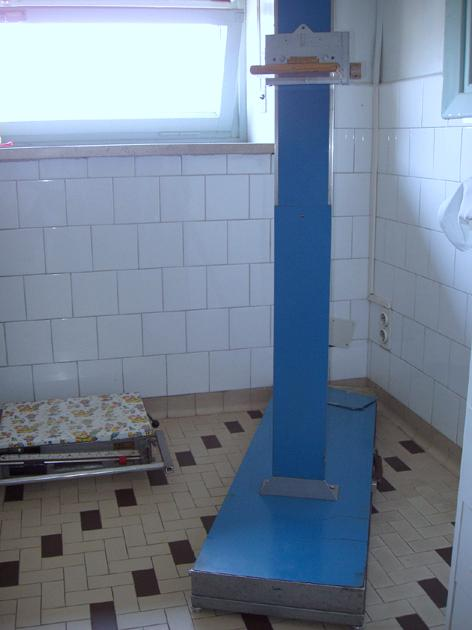
\includegraphics[scale=0.40]{grafici/statimetro.jpg}
  \end{center}
  \caption{Statimetro di Harpenden}
\end{figure}
La tecnica per il rilievo della statura da eretto è la seguente: il soggetto deve stare in piedi, con i talloni vicini fra loro e con i calcagni, le natiche e le spalle appoggiati al piano verticale dello statimetro. I piedi sono leggermente divaricati, in modo da formare un angolo di circa 45 gradi; il soggetto non indossa i propri calzini, ma un paio di sottili calzari in plastica, al fine di ridurre lo spessore. La testa viene orientata nella posizione di Francoforte. Al momento della misurazione il soggetto viene invitato a compiere un'inspirazione profonda, mentre l'osservatore lo tiene in distensione esercitando una trazione verso l'alto con il dito medio di ciascuna mano posto sotto i processi mastoidei. La statura si legge sull'apposito indicatore durante la successiva espirazione, mantenendo la pressione sotto i processi mastoidei%figure con Vannelli.

\subsubsection*{Peso}
Rappresenta l'insieme della massa magra e di quella adiposa. Deve essere rilevato mediante una bilancia tarata che assicuri un approssimazione di kg 0,1. Il soggetto viene pesato con il minimo di indumenti, possibilmente al mattino dopo aver urinato.

\subsubsection*{Velocità di crescita staturale}
Rappresenta l'accrescimento staturale avvenuto in un determinato periodo di tempo. Per calcolarla occorre dividere la differenza fra due misurazioni per l'intervallo di tempo fra queste misurazioni. L'intervallo non deve essere nè troppo breve nè molto lungo: in genere la velocità di crescita staturale si calcola su 6 mesi.

\subsubsection*{Stadi puberali}
Sono un'importante indicatore di maturazione nel periodo puberale\cite{benso2001auxologia}. Nei maschi si rilevano lo stadio dello sviluppo pilifero al pube e dello sviluppo dei genitali; nelle femmine lo sviluppo pilfero al pube e lo sviluppo mammario. Generalmente viene adottata la classificazione di Tanner\cite{tanner1990foetus} in cinque stadi.

\begin{table}[!h]
\begin{tabular}{lp{13.3cm}}
\toprule
\multicolumn{2}{c}{\textbf{Stadi dello sviluppo pilifero al pube (\emph{Pubic Hair})}}\\
PH1 &	preadolescente. Assenza di peli pubici o presenza di lieve peluria lanuginosa.\\
PH2 &	crescita sparsa dei primi peli lunghi, poco pigmentati che appaiono 
		in particolare alla base del pene o lungo le grandi labbra.\\
PH3 &	peli molto più scuri, più ruvidi e più crespi. 
		I peli si diffondono sparsi, sopra il pube.\\
PH4 &	i peli assomigliano al tipo proprio degli adulti ma non vi è diffusione 
		alla superficie mediale delle cosce.\\
PH5 &	configurazione da adulto per quantità e con distribuzione di tipo 
		orizzontale nelle femmine e diffusione lungo la linea
		alba nei maschi; diffusione alla superficie mediale delle cosce.\\
%\bottomrule
%\end{tabular}
%\label{tab:SviluppoPiliferoPube}
%\end{table}
%\begin{table}
%\begin{tabular}{lp{13.3cm}}
%\toprule
\midrule
\multicolumn{2}{c}{\textbf{Stadi dello sviluppo mammario (\emph{Breast})}}\\
B1 &	preadolescente: elevazione del solo capezzolo.\\
B2 &	sviluppo iniziale (bottone o gemma): lieve turgore della mammella \emph{in toto} e del capezzolo. 
		Aumento del diametro dell'areola rispetto allo stadio 1.\\
B3 &	ulteriore ingrandimento ed elevazione della mammella e dell'areola, senza separazione dei rispettivi contorni.\\
B4 &	elevazione dell'areola e dei capezzoli al di sopra del livello della mammella 
		(i contorni di areola e mammella sono netti).\\
B5 &	stadio della maturità. Proiezione del solo capezzolo, a causa 
		della scomparsa della distinzione fra contorno 
		dell'areola e contorno della mammella.\\
%\bottomrule
%\end{tabular}
%\label{tab:SviluppoMamario}
%\end{table}
%\begin{table}
%\begin{tabular}{lp{13.3cm}}
%\toprule
\midrule
\multicolumn{2}{c}{\textbf{Stadi dello sviluppo genitale maschile (\emph{Genitalia})}}\\
G1 &	preadolescente. Testicoli, scroto e pene sono all'incirca delle medesime dimensioni e proporzioni che si riscontrano nell'infanzia.\\
G2 &	aumento del volume dello scroto e dei testicoli. La cute dello scroto è rosseggiante e cambia di struttura. 
		Lieve o nessun aumento di dimensioni del pene.\\
G3 &	aumento delle dimensioni del pene, che riguardano dapprima sopprattutto la lunghezza.
		Testicoli e scroto sono aumentati rispetto allo stadio 2.\\
G4 &	aumento del pene, che cresce in senso trasversale e sviluppo del glande. Ulteriore aumento di volume dei testicoli e dello scroto; 
		aumentata pigmentazione della cute scrotale.\\
G5 &	genitali di tipo adulto per dimensioni e aspetto. Dopo questo stadio non si verifica altro accrescimento.\\
\bottomrule
\end{tabular}
%\label{tab:SviluppoGenitaleMaschile}
\end{table}

\clearpage

\begin{figure}[h]
  \begin{center}
      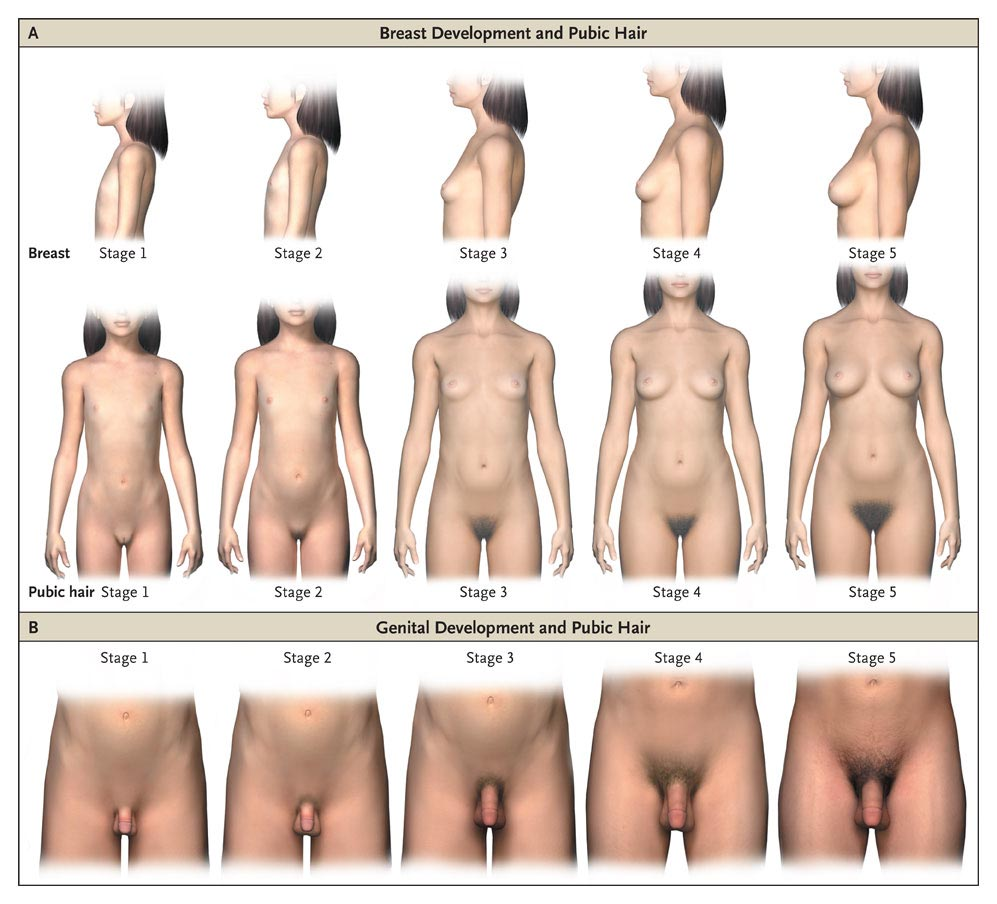
\includegraphics[scale=0.43]{grafici/Tanner_Stages} %\\
  \end{center}
  \caption{Stadi puberali secondo la classificazione Tanner.}
\end{figure}

\subsubsection*{Orchidometria}
Consiste nella valutazione del volume testicolare. A tale scopo viene utilzzato l'orchidometro di Prader %figura.
Le dimensioni dei testicoli sono valutate paragonandoli, mediante palpazione manuale, con dei modelli standard di dimensioni crescenti dell'orchidometro. Il valore di 4 ml è da considerarsi valore limite fra la preadolescenza e l'inizio della pubertà.  

\begin{figure}[h]
  \begin{center}
	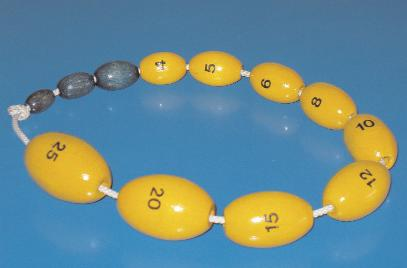
\includegraphics[scale=0.60]{grafici/orchidometro.jpg}
  \end{center}
  \caption{Orchidometro di Prader}
\end{figure}

\subsubsection*{Statura bersaglio}
Si tratta dell'altezza che ci si attende nella maggior parte dei figli sani di una coppia con una data statura. Il centro del bersaglio si ottiene nel modo seguente: per i maschi si sommano l'altezza del padre e quella della madre espressa al maschile (cioè si aggiungono 13 centimetri all'altezza materna, perchè tale è la differenza statistica fra maschi e femmine) e si divide il risultato per due; per le femmine si sommano l'altezza della madre e quella del padre espressa al maschile (vale a dire si sottraggono 13 centimetri alla statura paterna per il motivo sopra esposto) e si divide il risultato per due. 

Il centro del bersaglio $\pm$ 8 cm fornisce l'intervallo entro cui dovrebbe situarsi la maggior patre dei figli di una coppia con quella data statura.





\clearpage

\subsection{Valutazione ormonale}

Non esiste un \emph{gold standard} per la diagnosi di deficit nella produzione di GH\cite{gh2003update}. La sua secrezione, infatti, è un \emph{continuum} tra normalità e deficit grave. Pertanto i cut-off convenzionalmente usati sono arbitrari e, sebbene i bambini con grave deficit di GH non rispondano ai test di stimolo, non ci sono dubbi che alcuni bambini deficitari di GH ottengano concentrazioni di ormone somatotropo stimolate superiori ai limiti arbitrari applicati.
In passato (nota CUF 39) si parlava di deficit di GH a patogenesi ipofisaria qualora il soggetto non avesse risposto a due test provocativi classici (picco di GH inferiore ai 10 \unit{\micro g}/l dopo stimolo con arginina, glucagone o clonidina) oppure ad un test massimale con GHRH + arginina (picco inferiore a 20 \unit{\micro g}/l); il deficit era definito a patogenesi ipotalamica quando la secrezione somatotropa spontanea media era inferiore ai 3 \unit{\micro g}/l; si parlava di deficit di attività biologica del GH in presenza di bassi livelli di somatomedine (IGF-1) normoresponsivi al test di generazione somatomedinica in pazienti con normale secrezione somatotropa spontanea o stimolata.
L'attuale nota AIFA 39 (18/11/2010) non prende più in considerazione il deficit a patogenesi ipotalamica e quello di attività biologica, ma prevede il trattamento dei bambini nati SGA alle seguenti condizoni: il peso alla nascita deve essere inferiore al terzo centile o comunque al di sotto dei 2500 g; la statura all'inizio della terapia deve trovarsi a -2,5 DS dalla media e la velocità di crescita non deve superare il cinquantesimo centile; il trattamento deve avvenire non prima dei quattro anni di età; sono concessi per ora solo due anni di terapia, in quanto mancano studi che riportino l'impatto della terapia con rGH sulla statura finale dei bambini nati piccoli per l'età gestazionale.

\subsubsection*{L'arginina}
L'arginina è un aminoacido che stimola la secrezione di ormone della crescita verosimilmente inibendo la somatostaina ipotalamica. Viene infusa sottoforma di arginina cloridrato alla dose di 0,5 g/kg (fino ad un massimo di 30 g) in 30 minuti per via endovenosa. I prelievi ematici vengono attualmente effettuati a 0-30-60-90 minuti; precedentemente si eseguivano dopo 30-60-90-120 minuti. L'infusine di arginina non presenta effetti collaterali, esclusa una possibile reazione infiammatoria locale da stravaso.

\subsubsection*{Il glucagone}
Il glucagone stimola il rilascio di GH con meccanismo diretto, analogalmente ai peptidi GH liberatori ed indiretto, mediante induzione di ipoglicemia secondaria. Si somministrano 50 \unit{\micro g}/kg (fino ad un massimo di 1 mg) sottocute o intramuscolo. I prelievi ematici per dosare l'ormone della crescita oggi si effettuano a 0-60-90-120-150 minuti; precedentemente si esguivano a 90-120-150-180 minuti. La somministrazione di glucagone può provocare nausea, vomito; è bene fornire un pasto ricco di carboidrati alla fine del prelievo ematico per ridurre il rischio di ipoglicemia tardiva.

\subsubsection*{La clonidina}
La clonidina è un agonista alfa2adrenergico, che stimola i neuroni produttori di GHRH ed inibisce la secrezione ipotalamica di somatostatina. La si somministra per via orale, sciolta in acqua, alla dose di 0,1-0,5 mg/m2. I prelievi ematici si eseguono dopo 0-30-60-90-120 minuti; in passato si effettuavano dopo 30-60-90-120 minuti. La clonidina può dara effetti collaterali a volte anche gravi: ipotensione marcata, bradiaritmia, sonnolenza.
 
\subsubsection*{Il GHRH + arginina}
Il meccanismo d'azione è duplice: il GHRH induce la liberazione di ormone somatotropo, mentre l'arginina inibisce il rilascio di somatostatina. Si tratta di un test molto potente. L'arginina viene infusa come esposto sopra. Al termine dell'infusione si somministra un bolo di GHRH alla dose di 1 \unit{\micro g}/kg (fino ad un massimo di 50 \unit{\micro g}) per via endovenosa. I prelievi ematici per dosare l'ormone somatotropo vengono eseguiti a 0-30-90 minuti. Gli effetti collaterali sono scarsi; può comparire un transitorio rossore al volto.

\subsubsection*{La screzione somatotropa spontanea media}
La secrezione spontanea media viene generalmente valutata nelle 12 ore notturne con prelievi ematici ogni trenta minuti. Nei bambini della prima infanzia ed in quelli di età maggiore le cui condizioni cliniche non sono soddisfacenti, i prelievi possono essere eseguiti ad intervalli di un'ora.

\subsubsection*{La generazione somatomedinica}
Il test di generazione somatomedinica si effettua con la somministrazione di rGH sottocute alla dose di 0,1 U.I./kg per quattro sere consecutive alle ore 21. La risposta al test è normale quando il valore di IGF-1 dopo rGH esogeno aumenta almeno del 50 \%
rispetto al valore basale.



\subsection{Analisi statistiche}
